\documentclass[12pt]{article}
\usepackage{geometry}                % See geometry.pdf to learn the layout options. There are lots.
\geometry{letterpaper}                   % ... or a4paper or a5paper or ... 
%\geometry{landscape}                % Activate for for rotated page geometry
\usepackage[parfill]{parskip}    % Activate to begin paragraphs with an empty line rather than an indent
\usepackage{daves,fancyhdr,natbib,graphicx,dcolumn,amsmath,lastpage,url}
\usepackage{amsmath,amssymb,epstopdf,longtable}
\usepackage{paralist}  % need to modify standard enumerate blocks
\DeclareGraphicsRule{.tif}{png}{.png}{`convert #1 `dirname #1`/`basename #1 .tif`.png}
\pagestyle{fancy}
\lhead{CE 3354 -- Engineering Hydrology}
\rhead{SUMMER 2025}
\lfoot{EX1}
\cfoot{}
\rfoot{Page \thepage\ of \pageref{LastPage}}
\renewcommand\headrulewidth{0pt}



\begin{document}
\begin{center}
{\textbf{{ CE 3354 Engineering Hydrology} \\ {Exam 1}}}
\end{center}


\begin{enumerate}

\item For a watershed with a size of $120~km^2$, the following data on precipitation $P$, evaporation
$E$ and runoff $Q$ are recorded in watershed mm.

\begin{table}[h!]
\centering
\caption{Monthly Precipitation (P), Evapotranspiration (E), and Runoff (Q)}
\begin{tabular}{|c|cccccccccccc|}
\hline
\textbf{Month} & Jan & Feb & Mar & Apr & May & Jun & Jul & Aug & Sep & Oct & Nov & Dec \\
\hline
\textbf{P (mm)} & 250 & 205 & 165 & 50 & 5 & 0 & 0 & 5 & 10 & 55 & 65 & 190 \\
\textbf{E (mm)} & 5 & 25 & 30 & 50 & 80 & 100 & 150 & 70 & 60 & 20 & 10 & 5 \\
\textbf{Q (mm)} & 150 & 110 & 80 & 5 & 0 & 0 & 0 & 0 & 0 & 10 & 15 & 120 \\
\hline
\end{tabular}
\end{table}

Determine:
    \begin{enumerate}[a)]
        \item The month (end) when the amount of water stored in the basin is the largest. 
        \item The month (end) when the amount of water stored in the basin is the smallest.
        \item The difference (in $m^3$) in the amount of water stored in the basin between these
two extremes.
        \item The likely climate type (arid, humid temperate or humid tropical) one would expect to find this
catchment.
    \end{enumerate}

\textbf{Solution(s)}:
Items a,b, and c are determined using a water budget approach.  An excel spreadsheet is shown in Figure(s) \ref{fig:pr1_xls}, and \ref{fig:pr1_form}

\begin{figure}[h!] %  figure placement: here, top, bottom, or page
   \centering
   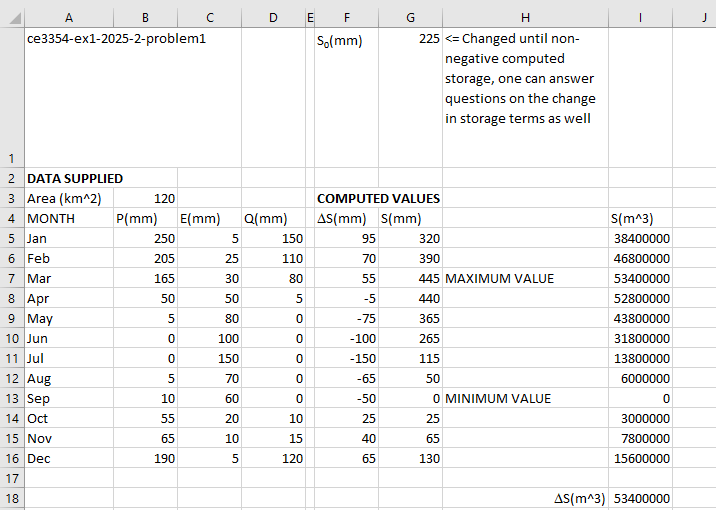
\includegraphics[width=6in]{pr1_xls.png} 
   \caption{PR1 Water Budget}
   \label{fig:pr1_xls}
\end{figure}

\begin{figure}[h!] %  figure placement: here, top, bottom, or page
   \centering
   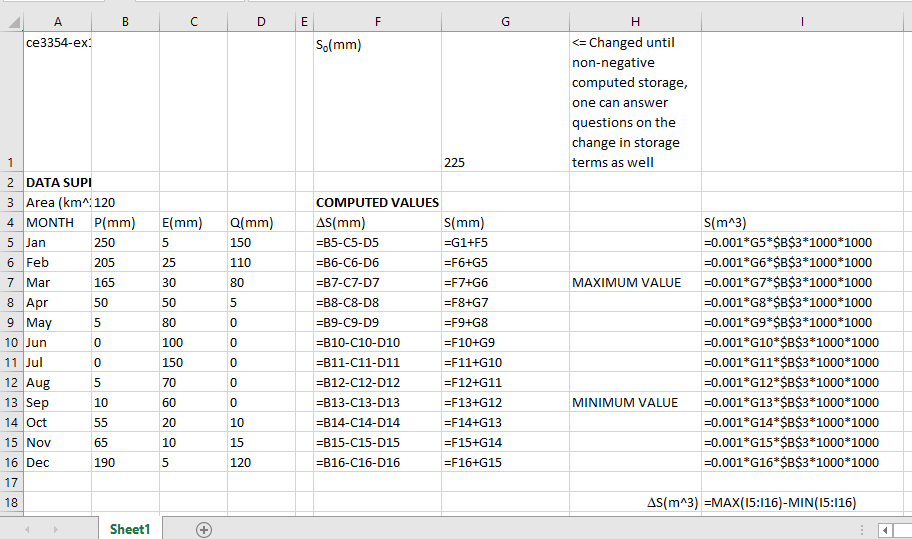
\includegraphics[width=6in]{pr1_form.png} 
   \caption{PR1 Water Budget Formulas}
   \label{fig:pr1_form}
\end{figure}

\clearpage
Item d requires internet research to learn about climate classification.  The model I used is \textsl{Köppen climate classification}, Gupta's classification(s), and Mays' classifications follow closely.  A good starting place is Wikipedia \url{https://en.wikipedia.org/wiki/Köppen_climate_classification}.

For the supplied monthly values we can make the following assertions:
\begin{itemize}
\item Rainfall (P) is highly concentrated in Jan–Mar and Dec.
\item Dry season from May–Sep (very low P, high E).
\item E is high in May–Sep, reaching a peak in July (150 mm) when P is 0.
\end{itemize}

These data indicate a distinct wet/dry seasonality.

The Köppen classification scheme:
\begin{itemize}
\item Distinct wet and dry seasons
\item Wet summer is not present — rainfall is in winter.
\item Dry summer with high E
\item Total annual precipitation is moderate (1000 mm)
\end{itemize}

This pattern is typical of a Mediterranean Climate (Köppen: Csa or Csb)
Csa: Hot, dry summer; mild, wet winter (likely match)

Characteristics:
\begin{itemize}
\item Summer drought
\item 3+ months with P $<$ 30 mm and E $>$ 60 mm (May–Sep fits)
\item Wet winters (P $>$ E in Jan–Mar, Dec)
\end{itemize}

The catchment is most likely in a Mediterranean climate (Köppen Csa), common in:

\begin{itemize}
\item Coastal California
\item Southern Europe (e.g., Spain, Italy)
\item Western Australia
\item Cape region of South Africa
\item Parts of central Chile
\end{itemize}

\clearpage
%%%%%%%%%%%%%%%%%%%%%%%%%%%%%%%%%%%%%%%%%%%%%%%%%%%%%%%%%%%%
\item A watershed with a catchment area of 1$mi^2$ converts about 60-percent of precipitation into streamflow, the remainder is lost.  The watershed response equation is 

\begin{equation}
 k\frac{dQ}{dt} + Q(t) = P(t) \cdot A \cdot C 
\end{equation}

where $Q(t)$ is the streamflow leaving the catchment, $P(t)$ is the precipitation entering the catchment, $A$ is the catchment area, $C$ is the precipitation to streamflow conversion fraction, and $k$ is the basin characteristic time constant.

\begin{figure}[h!] %  figure placement: here, top, bottom, or page
   \centering
   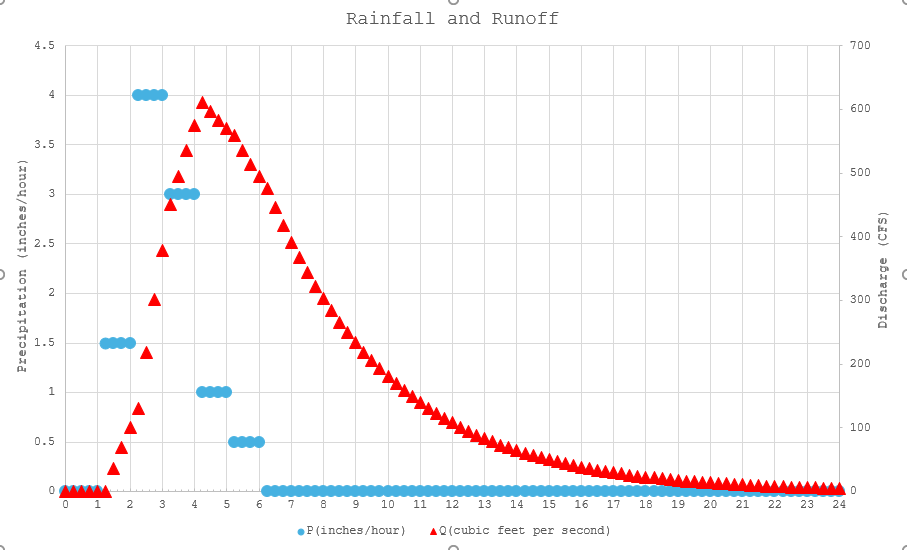
\includegraphics[width=6in]{EX1-P2_PLOT.png} 
   \caption{Rainfall-runoff plot for the catchment}
   \label{fig:EX1-P2-PLOT}
\end{figure}

Using the information in Figure \ref{fig:EX1-P2-PLOT} determine:

    \begin{enumerate}[a)]
        \item The maximum discharge rate in cubic feet per second.
        \item The time when the maximum discharge occurs.
        \item The value in hours of the of the basin time constant $k$.
        \item The total volume in acre feet of precipitation entering the catchment (before any losses)
        \item The total volume in acre feet of discharge leaving the catchment 
    \end{enumerate}
\clearpage
\textbf{Solution(s)}:
Items a, and b can be read directly from the supplied plot.  They are about 600 cfs and 4.25 hours.  We can get more accurate estimates when we simulate the watershed using the supplied equation, and fit the simulated chart to the provided chart.

To fit fisrt build a finite-difference approximation as

$k\frac{dQ}{dt} + Q(t) = P(t)\cdot A \cdot C$  

$A$ should be supplied in acres assuming $P \cdot C$ is in inches per hour to produce output in CFS.

Move $Q(t)$ to RHS and divide by $k$

$\frac{dQ}{dt}  = \frac{P(t)\cdot A \cdot C-Q(t)}{k}$

Then express the LHS as a difference quotient

$\frac{Q(t+\Delta t) - Q(t)}{\Delta t}  = \frac{P(t)\cdot A \cdot C-Q(t)}{k}$

Isolate everything at the old time step to the RHS

$Q(t+\Delta t)  = Q(t)  + \frac{\Delta t}{k} (P(t)\cdot A \cdot C-Q(t))$

Code up into a spreadsheet, choose a small enough value of $\Delta t$ and proceede.

Figure \ref{fig:pr2_xls} is a screen capture of a portion of the spreadsheet.

\begin{figure}[h!] %  figure placement: here, top, bottom, or page
   \centering
   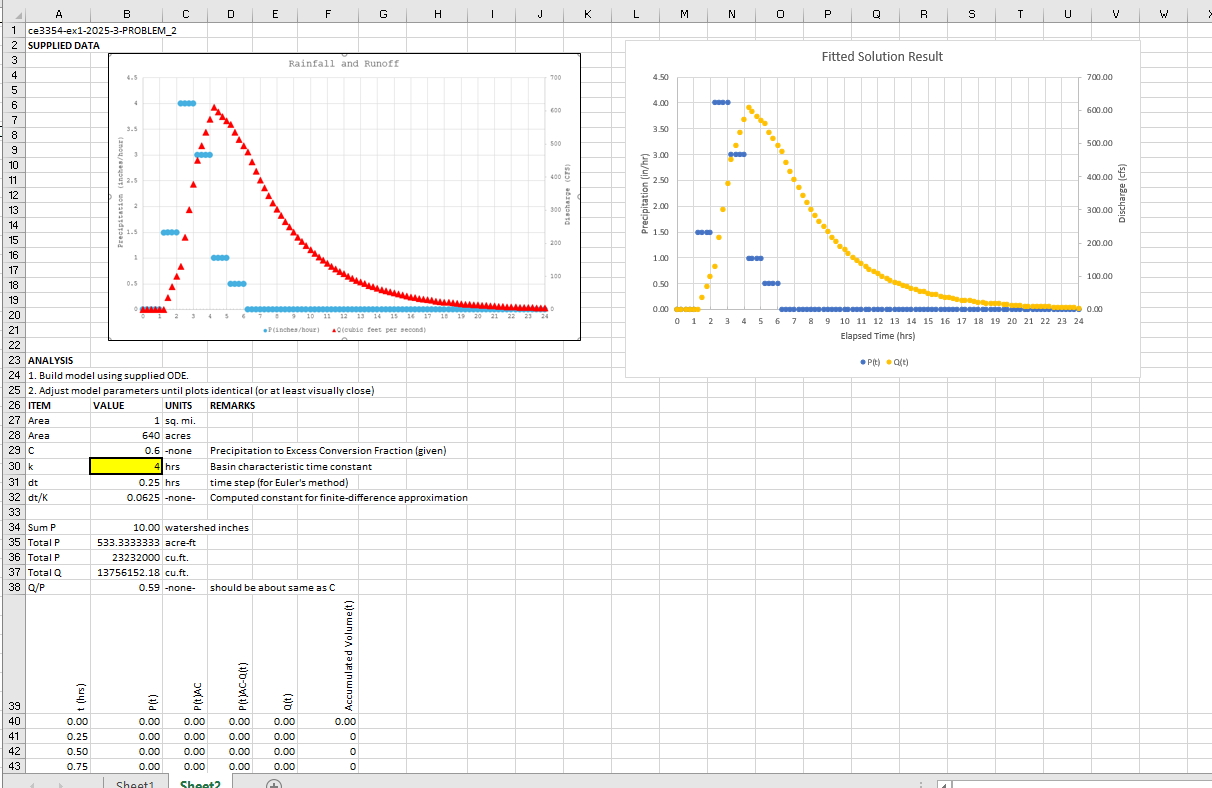
\includegraphics[width=6in]{pr2_xls.png} 
   \caption{Rainfall-runoff plot for the catchment; supplied and computed charts side-by-side}
   \label{fig:pr2_xls}
\end{figure}
\clearpage
Figure \ref{fig:pr2_calcs} is a screen capture of the computation portion of the spreadsheet.

\begin{figure}[h!] %  figure placement: here, top, bottom, or page
   \centering
   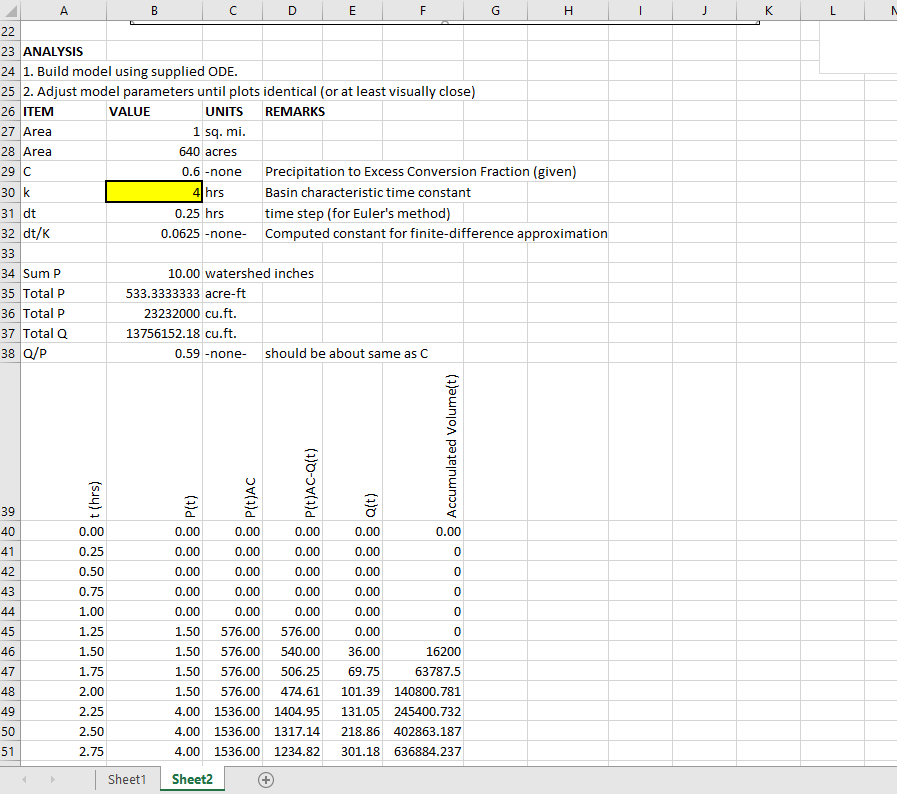
\includegraphics[width=6in]{pr2_calcs.png} 
   \caption{Rainfall-runoff plot for the catchment; calculation portion.  $k$ is fit by trial-and-error updating}
   \label{fig:pr2_calcs}
\end{figure}

To demonstrate quality of the simulation, we change the computed chart background to transparent and overlay it onto the supplied graphic element.  Figure \ref{fig:pr2_overlay} is the result.  It is evident the fit is exact.

\begin{figure}[h!] %  figure placement: here, top, bottom, or page
   \centering
   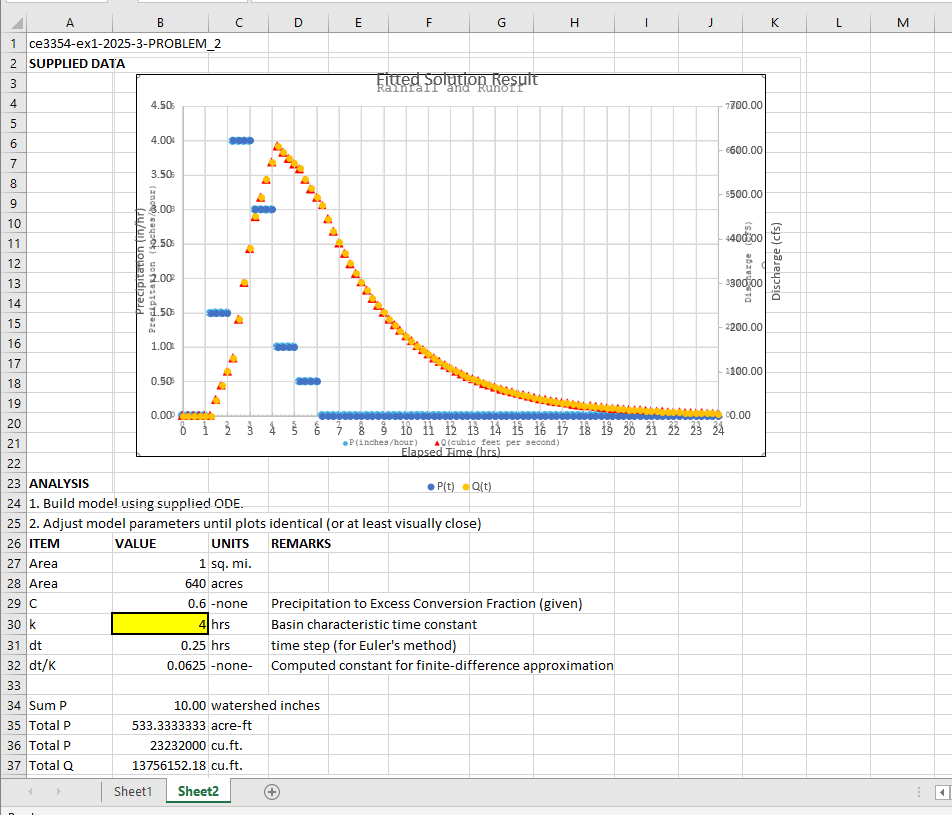
\includegraphics[width=6in]{pr2_overlay.png} 
   \caption{Rainfall-runoff plot for the catchment; Computed plot overlay and scaled so axes are same range.}
   \label{fig:pr2_overlay}
\end{figure}
\clearpage
Items c,d, and e appear directly or are computed from summary values in Figure \ref{fig:pr2_calcs}.

c) value of $k$ is 4 hours (to obtain the fitted chart)

d) Total volume in acre-feet of precipitation is \textbf{533.33 acre-feet}

e) Total volume in acre feet of runoff is 13,756,152 cu.ft. divided by 43560 sq. ft./acre-ft to obtain \textbf{315.80 acre-feet}.

Lastly Figure \ref{fig:pr2_forms} is a portion of the spreadsheet showing the formulas employed.

\begin{figure}[h!] %  figure placement: here, top, bottom, or page
   \centering
   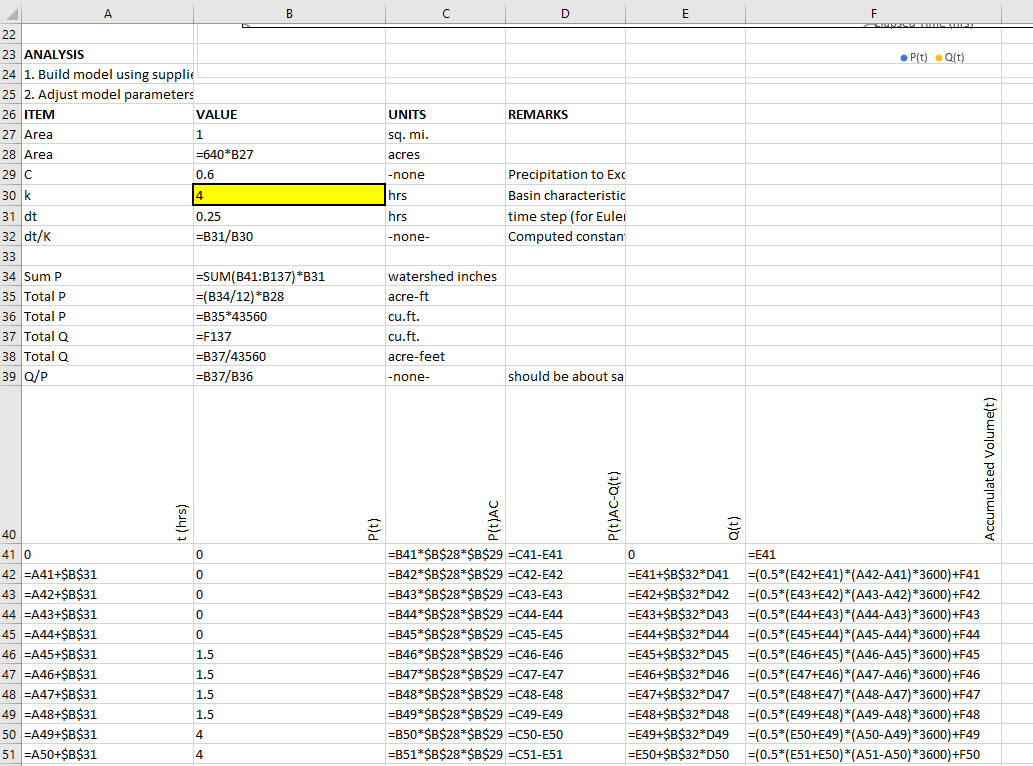
\includegraphics[width=6in]{pr2_forms.png} 
   \caption{Rainfall-runoff formulas for the catchment}
   \label{fig:pr2_forms}
\end{figure}


\clearpage
%%%%%%%%%%%%%%%%%%%%%%%%%%%%%%%%%%%%%%%%%%%%%%%%%%%%%%%%%%%%
\item Using an appropriate NRCS 24-hour rainfall distribution

Determine:
    \begin{enumerate}[a)]
        \item The cumulative rainfall depth (inches) for a 50-yr ARI storm in Lubbock, Texas.
        \item The rainfall intensity (inches/hour) for each half-hour increment of the storm. 
        \item The maximum rainfall intensity (inches/hour) in any 30-minute interval.  
    \end{enumerate}

\textbf{Solution(s)}:
An apropriate NRCS distribution for Lubbock, Texas is a Type-II storm. Figure \ref{fig:pr3_map} is a screen capture of a map showing that Lubbock is best reperesented by Type II.

\begin{figure}[h!] %  figure placement: here, top, bottom, or page
   \centering
   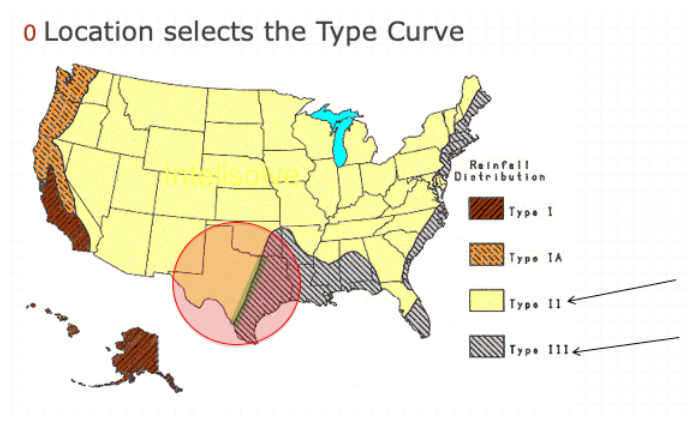
\includegraphics[width=5in]{pr3_map.png} 
   \caption{NRCS Type Curve Map}
   \label{fig:pr3_map}
\end{figure}

\clearpage

Item a) use NRCS PFDS to look up 24-hr storm depth. Using Partial Duration Series for Lubbock, TX value is \textbf{6.09 inches}.  Figure \ref{fig:pr3_pfds} is a screen capture of the NRCS server access.

\begin{figure}[h!] %  figure placement: here, top, bottom, or page
   \centering
   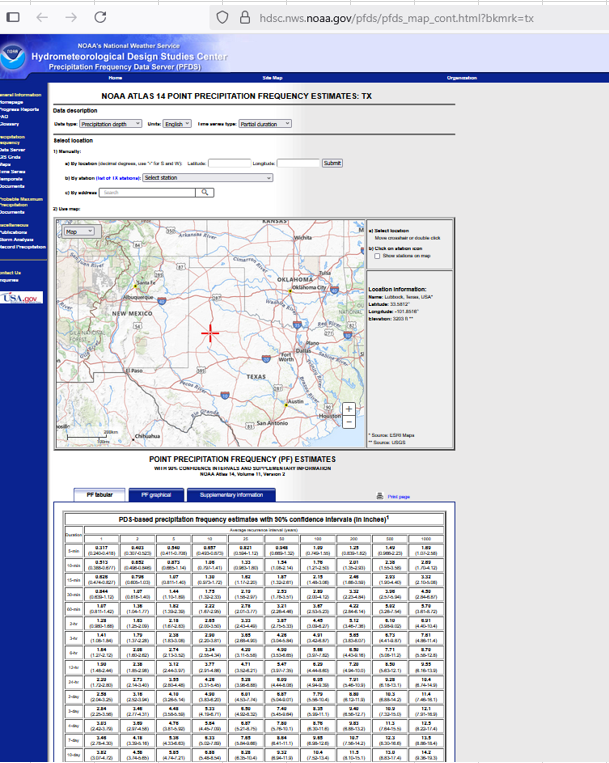
\includegraphics[width=5in]{pr3_pfds.png} 
   \caption{PFDS lookup for Lubbock, Texas}
   \label{fig:pr3_pfds}
\end{figure}

\clearpage
Item b) Use Script in notes, or spreadsheet implementation to obtain cumulative depth estimates each 1/2 hour.  Backward difference to obtain intensity.  Figure \ref{fig:pr3_script} is a screen capture of the python script for processing design storms (provided in course notes, and es2 solution file).

\begin{figure}[h!] %  figure placement: here, top, bottom, or page
   \centering
   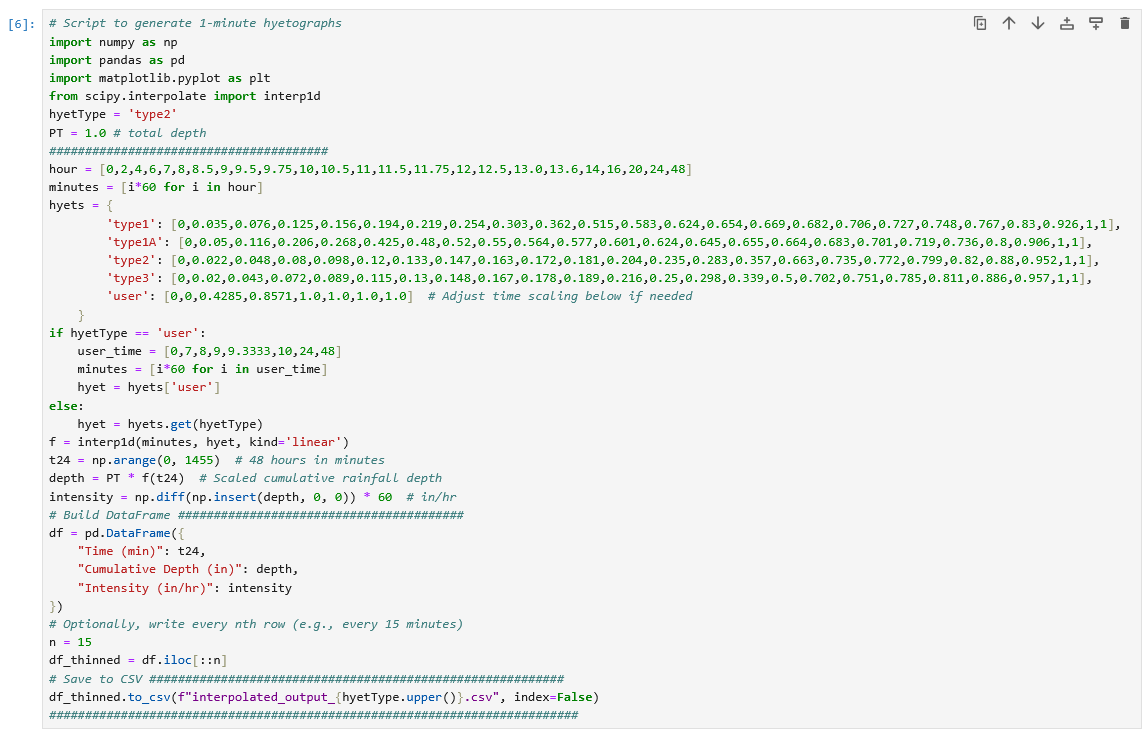
\includegraphics[width=5in]{pr3_script.png} 
   \caption{Script to generate Type II storm weights every 15 minutes}
   \label{fig:pr3_script}
\end{figure}

The output of the script is loaded into a spreadsheet to make the necessary computations to answer the remaining items.  Figure \ref{fig:pr3_xls} is a screen capture of such a spreadsheet.

\begin{figure}[h!] %  figure placement: here, top, bottom, or page
   \centering
   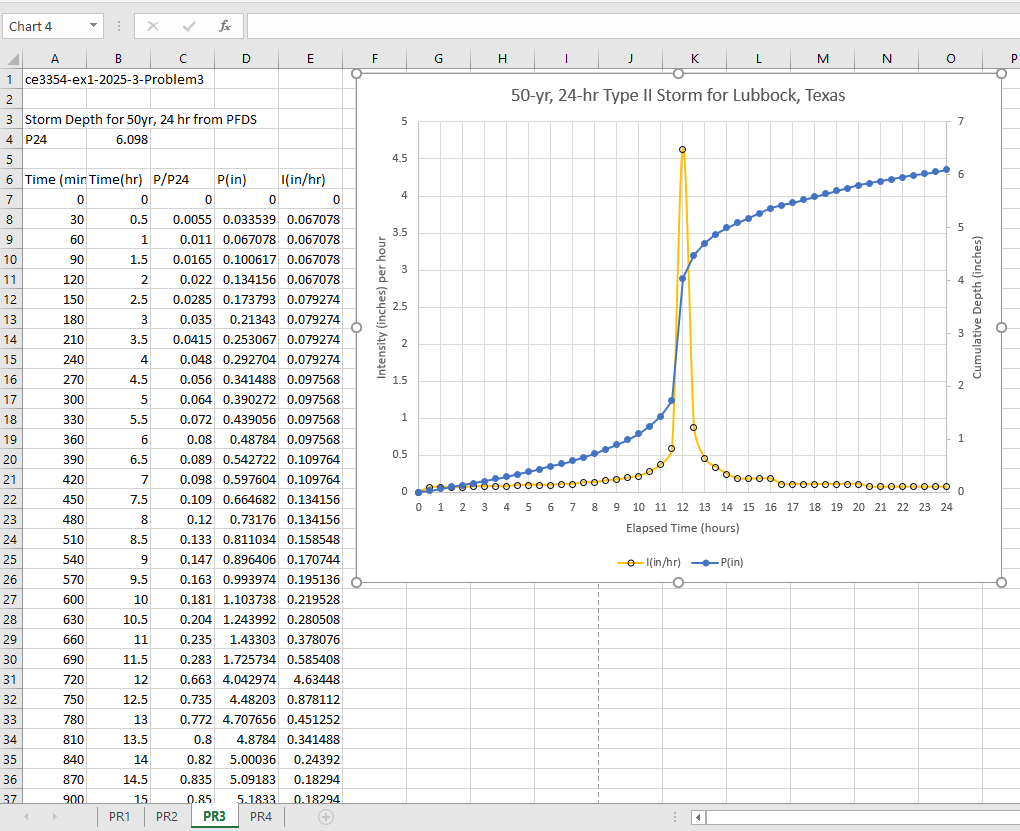
\includegraphics[width=5in]{pr3_xls.png} 
   \caption{Spreadsheet showing scaled storm depths and intensities (backward differences) for Type II storm. The differencing was performed in the python pre-processing script - all the spreadsheet does is rescale the results.}
   \label{fig:pr3_xls}
\end{figure}

Item b) based on differencing an interpolated NRCS storm, the intensity for each 1/2 hour is the column labeled I(in/hr) (rightmost in the figure), the maximum value in the spreadsheet, Item c) is 7.46 in/hr.\footnote{If you did not actually make the calculations and instead just reported the 30-min intensity from the PFDS, that value is 5.04 in/hour -- partial credit for reporting this value}

Figure \ref{fig:pr3_xls} is a screen capture of the spreadsheet as formulas.

\begin{figure}[h!] %  figure placement: here, top, bottom, or page
   \centering
   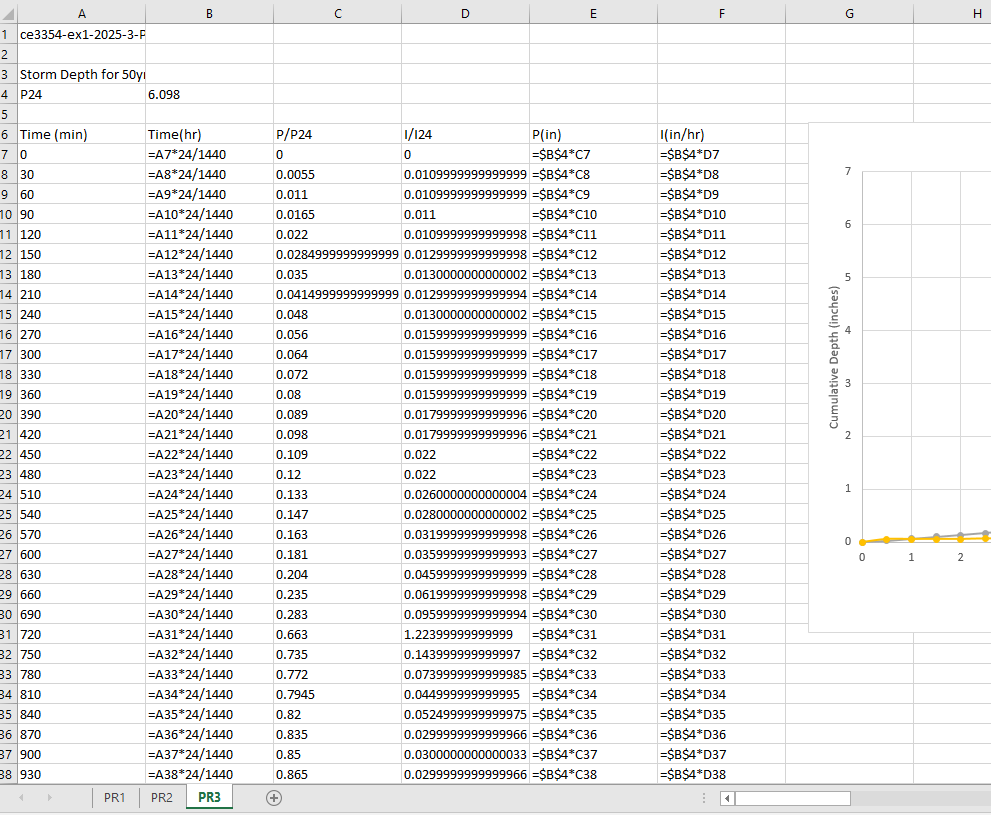
\includegraphics[width=5in]{pr3_forms.png} 
   \caption{Spreadsheet showing scaled storm depths and intensities formulas for Type II storm}
   \label{fig:pr3_forms}
\end{figure}

\clearpage
%%%%%%%%%%%%%%%%%%%%%%%%%%%%%%%%%%%%%%%%%%%%%%%%%%%%%%%%%%%%
\item The relation between infiltration capacity in mm/hour and the time (in hours) since the
start of the experiment as measured with an infiltrometer is depicted in Figure \ref{fig:INFIL}. 

\begin{figure}[h!] %  figure placement: here, top, bottom, or page
   \centering
   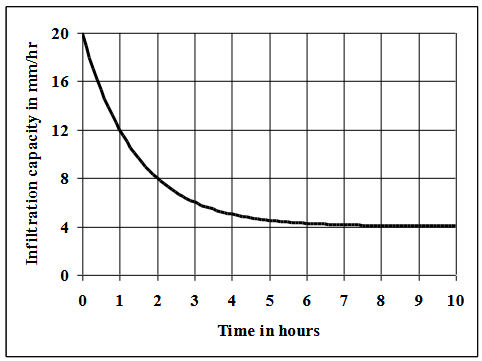
\includegraphics[width=5in]{INFIL.png} 
   \caption{Infiltrometer data for some soil}
   \label{fig:INFIL}
\end{figure}

The relationship is to be described with the Horton infiltration model 
\begin{equation}
q(t)=f_c+(f_o-f_c)e^{-kt}
\end{equation}

Determine:
    \begin{enumerate}[a)]
        \item The equilibrium infiltration rate, $f_c$, in mm/hr.
        \item The initial (dry soil) infiltration rate, $f_o$, in mm/hr.
        \item The soil constant $k$.
        \item The total amount of water that will infiltrate into an initially dry soil during a rainstorm with a duration 60 minutes and a constant intensity of 20 mm/h.
        \item The total amount of water that will infiltrate into an initially dry soil during a rainstorm with a duration 480 minutes and a constant intensity of 12 mm/h.
    \end{enumerate}

\textbf{Solution(s)}:

Use ES3 solution to construct a spreadsheet and fit infiltration curve as shown in Figure \ref{fig:pr4_xls_one}

\begin{figure}[h!] %  figure placement: here, top, bottom, or page
   \centering
   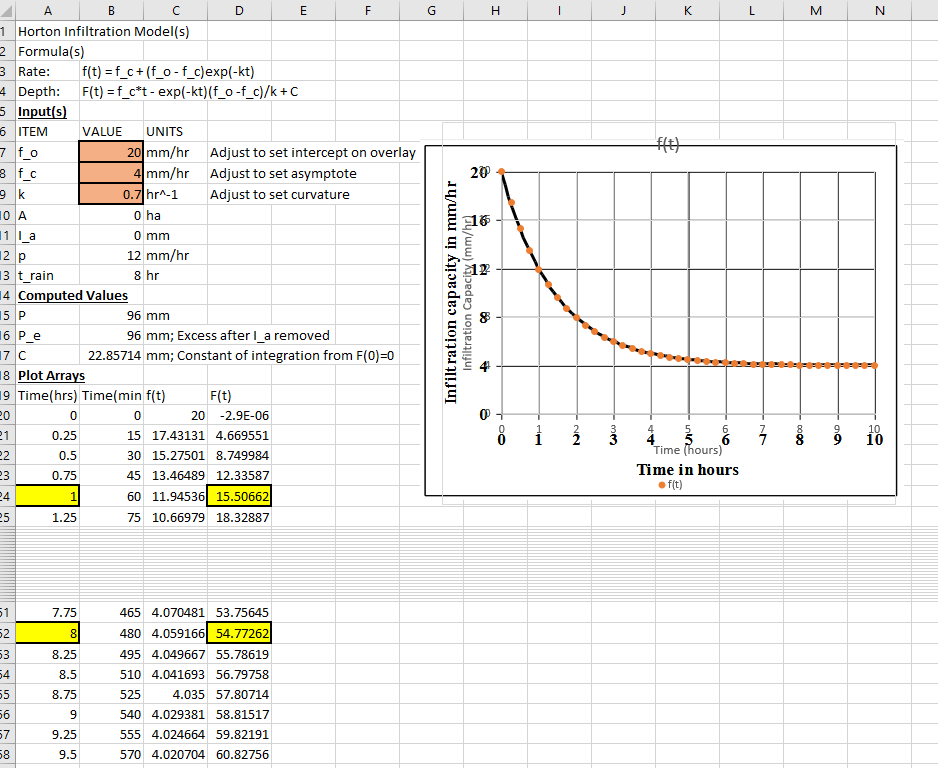
\includegraphics[width=5in]{pr4_xls_one.png} 
   \caption{Fitted Infiltrometer data for some soil on es3 solution spreadsheet tool.  Change chart background to transparent, and overlay, resize to fit provided curve.}
   \label{fig:pr4_xls_one}
\end{figure}

Results are:

    \begin{enumerate}[a)]
        \item The equilibrium infiltration rate, $f_c$, is $4.0~mm/hr$.
        \item The initial (dry soil) infiltration rate, $f_o$, is $20.0~mm/hr$.
        \item The soil constant $k$, is $0.7~\frac{1}{hr}$.
        \item The total amount of water that will infiltrate into an initially dry soil during a rainstorm with a duration 60 minutes and a constant intensity of 20 mm/h is $15.5~mm$.
        \item The total amount of water that will infiltrate into an initially dry soil during a rainstorm with a duration 480 minutes and a constant intensity of 12 mm/h is $54.7~mm$
    \end{enumerate}

\end{enumerate}



\end{document}  